\chapter{Uma iniciação à Teoria dos Grafos}

Capítulo 2 de Szwarcfiter, \textit{Grafos e Algoritmos Computacionais}~\cite{Szwarcfiter1986grafos}.

%%%%%%%%%%%%%%%%%%%%%%%%%%%%%%%%%%%%%%%%%%%%%%%%%%%%%%%%%%%%
\section{Introdução}

Serão dadas neste capítulo algumas definições de Teoria dos Grafos.

%%%%%%%%%%%%%%%%%%%%%%%%%%%%%%%%%%%%%%%%%%%%%%%%%%%%%%%%%%%%
\section{Os primeiros conceitos}

\begin{easylist}
& Grafo: representado por $G(V,E)$, é um conjunto finito não vazio $V$ e um conjunto $E$ de pares não ordenados de elementos distintos de $V$. Ver Figura~\ref{fig:1}.
\end{easylist}


\begin{figure}[b]
  \begin{center}
    \begin{tabular}{c}
      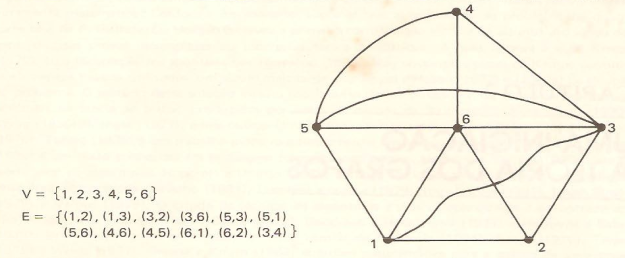
\includegraphics[width=0.7\textwidth]{images/02/fig1.png}
    \end{tabular}
  \end{center}
  \caption{\label{fig:1} Um grafo $G(V,E)$ e sua representação geométrica.}
  \source{Szwarcfiter~\cite{Szwarcfiter1986grafos}.}
\end{figure}


\begin{easylist}
& Vértices: são os elementos de $V$.
& Arestas: são os elementos de $E$.
& Grafo trivial: é um grafo onde $|V| = 1$.
& Vértices adjacentes: dois vértices $v, w$ são ditos adjacentes quando existe uma aresta $e$ tal que $e = (v, w)$; em outras palavras, quando alguma aresta incide em $v$ e $w$.
& Arestas adjacentes: são arestas que possuem uma extremidade em comum, ou seja, que incidem em algum vértice em comum.
& Isomorfismo entre grafos: dois grafos $G_1(V_1, E_1)$ e $G_2(V_2, E_2)$, com $|V_1| = |V_2|$, são ditos isomorfos se e somente se (sse) existe uma função bijetora $f:V_1 \mapsto V_2$ tal que $(v, w) \in E_1$ sse $(f(v), f(w)) \in E_2$ para todo $v, w \in V_1$. Ver Figura~\ref{fig:2}.
\end{easylist}


\begin{figure}[hb]
  \begin{center}
    \begin{tabular}{c}
      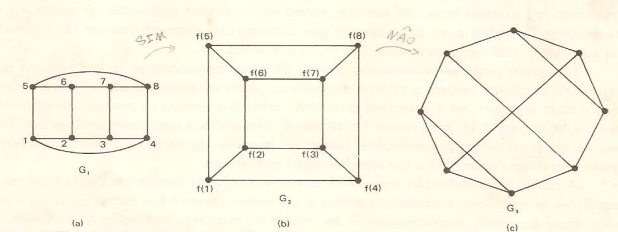
\includegraphics[width=0.8\textwidth]{images/02/fig2.png}
    \end{tabular}
  \end{center}
  \caption{\label{fig:2} Os grafos $G_1$ e $G_2$ são isomorfos um ao outro, mas não a $G_3$.}
  \source{Szwarcfiter~\cite{Szwarcfiter1986grafos}.}
\end{figure}


\begin{easylist}
& Grafo com laços: $G(V,E)$ é um conjunto finito não vazio $V$ e um conjunto $E$ de pares não ordenados de elementos de $V$.
& Grafo dirigido: $G(V,E)$ é um conjunto finito não vazio $V$ e um conjunto $E$ de pares ordenados de elementos de $V$.
& Multigrafo: $G(V,E)$ é um conjunto finito não vazio $V$ e um multiconjunto $E$ de pares não ordenados de elementos de $V$.

& Grau de um vértice $v$ é o número de arestas que incidem em $v$. Laços são contados duas vezes. É denotado por $\operatorname{grau}(v)$.
& Vértice isolado: é um vértice com grau zero.
& Grafo regular de grau $r$: é um grafo em que todos os vértices possuem o mesmo grau $r$.

& Caminho: uma sequência de vértices $v_1, \dots, v_k$ tal que $(v_i, v_{i+1}) \in E, 1\leq i < k$ é denominada caminho de $v_1$ a $v_k$. Seu comprimento é $k-1$.
& Alcance: dizemos que um vértice $v$ alcança um vértice $w$ se existe um caminho de $v$ a $w$.
& Caminho simples: caminho onde todos os vértices de $v_1$ a $v_k$ são diferentes.
& Trajeto: caminho onde todas as arestas são distintas.
& Ciclo: é um caminho $v_1, \dots, v_{k+1}$ em que $v_1 = v_{k+1}$ e $k \geq 3$.
& Ciclo simples: é um ciclo onde todos os vértices são diferentes, exceto o primeiro e o último.
& Grafo acíclico: é um grafo que não possui ciclos simples.
& Ciclos idênticos: ciclos obtidos um do outro por uma rotação de seus vértices.
& Caminho Hamiltoniano: caminho que contém cada vértice do grafo exatamente uma vez.
& Ciclo Hamiltoniano: ciclo $v_1, \dots, v_{k+1}$ onde o caminho $v_1, \dots, v_k$ é Hamiltoniano.
& Caminho ou ciclo Euleriano: caminho ou ciclo que contém cada aresta do grafo exatamente uma vez.
  
  
\begin{figure}[!h]
  \begin{subfigure}{.5\textwidth}
    \centering
    \begin{tabular}{c}
      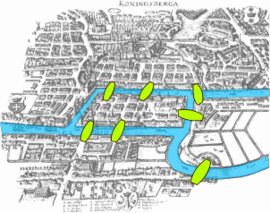
\includegraphics[width=1\textwidth]{images/02/Konigsberg_bridges.png}
    \end{tabular}
    \caption{\label{fig:kon:bridges} Pontes de Konigsberg.}
  \end{subfigure}
  \begin{subfigure}{.5\textwidth}
    \centering
    \begin{tabular}{c}
      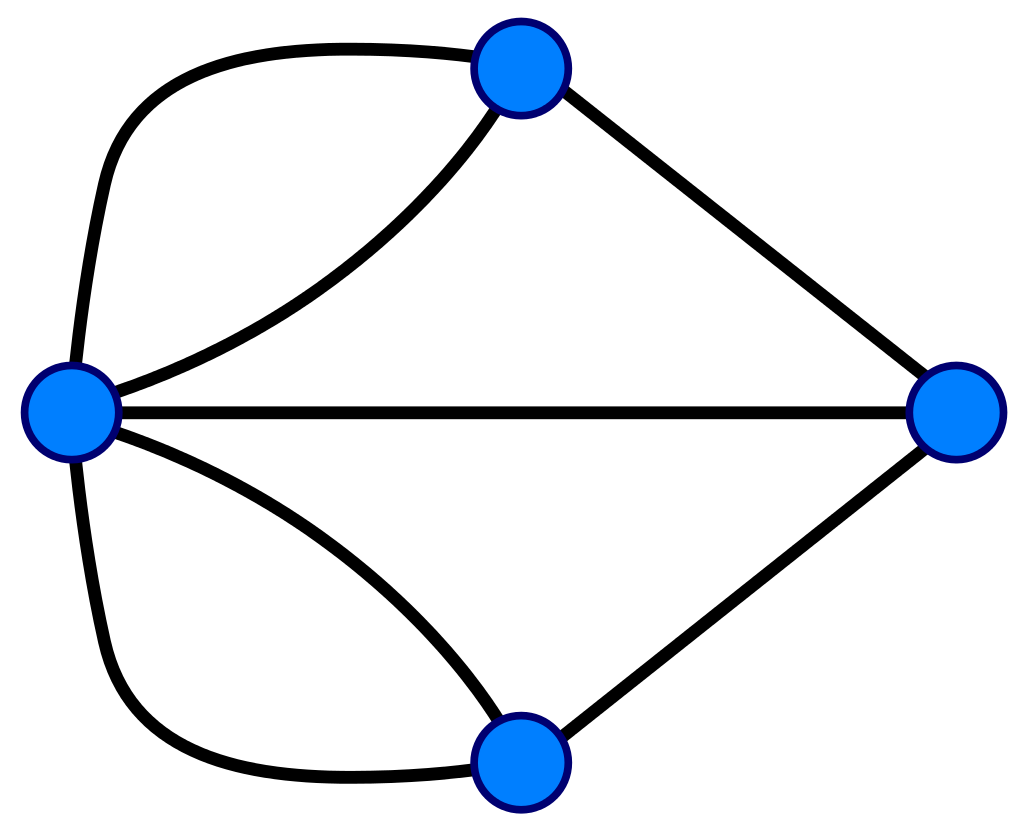
\includegraphics[width=1\textwidth]{images/02/Konigsberg_graph_svg.png}
    \end{tabular}
    \caption{\label{fig:kon:graph} Representação geométrica.}
  \end{subfigure}
  \caption{\label{fig:gray} Existe caminho que percorra todas as pontes uma única vez?}
  \source{Wikipedia.}
\end{figure}


& Grafo conexo: grafo onde, entre cada par de vértices, existe um caminho.
& Grafo desconexo: grafo que não é conexo. Em outras palavras, grafo em que existe algum par de vértices entre os quais não existe caminho.
& Grafo totalmente desconexo: grafo que não possui arestas.
& Subconjunto maximal em relação à propriedade $P$: seja $S$ um conjunto e $S' \subseteq S$, $S'$ é dito maximal em relação à propriedade $P$ quando $S'$ satisfaz $P$ e não existe subconjunto $S'' \supset S'$ que satisfaça $P$.
& Componente conexo: subgrafo de um grafo $G$ maximal com relação à conectividade.
& Subconjunto minimal em relação à propriedade $P$: definido de forma análoga ao subconjunto maximal.
& Distância entre dois vértices $v$ e $w$: denotada por $d(v, w)$ é o comprimento do menor caminho entre $v$ e $w$.

% Página 3

& Subtração e adição de vértices e arestas: seja $G(V, E)$ um grafo.
&& Seja $e \in E$ uma aresta, denota-se por $G - e$ o grafo obtido de $G$ pela exclusão da aresta $e$.
&& Seja $(v, w)$ um par de vértices não adjacentes de $G$, denota-se por $G + (v, w)$ o grafo obtido de $G$ adicionando-se a aresta $(v, w)$.
&& Seja $v \in V$ um vértice, denota-se por $G - v$ o grafo obtido da remoção do vértice $v$ e de todas as arestas nele incidentes.
&& Seja $v \notin V$ um vértice, denota-se por $G + v$ o grafo obtido de $G$ adicionando-se o vértice $v$.

& Teorema 2.1: um grafo conexo $G$ possui ciclo Euleriano sse todo vértice de $G$ possui grau par.
&& $\Rightarrow$ Seja $C$ um ciclo Euleriano de $G$. Para cada ocorrência de um vértice $v$ em $C$, somamos 2 a seu grau pelo fato de uma ocorrência corresponder a uma aresta de entrada e uma de saída. Portanto, todo vértice de $G$ possui grau par.
&& $\Leftarrow$ Assuma que todos os vértices de $G$ têm grau par. Começamos de um vértice arbitrário $v$ e percorremos um ciclo começando e terminando em $v$, sem repetir arestas. Se todas as arestas foram visitadas, então $G$ é Euleriano. Se não, removemos de $G$ as arestas pertencentes a $C$ e vértices isolados após a remoção, ficando com o grafo $G'$. Todos os vértices de $G'$ têm grau par. Partimos então de algum vértice $u \in G'$ pertencente ao ciclo $C$ e percorremos outro ciclo. O processo é repetido até que o grafo fique vazio. Um ciclo Euleriano pode ser obtido da concatenação de todos os ciclos encontrados. Portanto, $G$ possui ciclo Euleriano. $\QED$

& Grafo completo: é um grafo que possui uma aresta entre cada par de seus vértices. É denotado por $K_n$, onde $n = |V|$. Possui ${n}\choose{2}$ arestas.
& Complemento de um grafo $G(V, E)$: é o grafo $\bar{G}$ que também possui $V$ como conjunto de vértices e possui como conjunto de arestas $V^2 - E$, onde $V^2$ denota o conjunto de todos os pares não ordenados de elementos distintos de $V$.
& Grafo bipartido: um grafo $G(V, E)$ é bipartido quando seu conjunto de vértices pode ser particionado em dois conjuntos $V_1$ e $V_2$, tais que toda aresta incide em um vértice de $V_1$ e em um vértice de $V_2$.
& Grafo bipartido completo: possui uma aresta para par de vértices $(v_1, v_2)$, onde $v_1 \in V_1$ e $v_2 \in V_2$. É denotado por $K_{n_1, n_2}$, onde $n_1 = |V_1|$ e $n_2 = |V_2|$. Possui $n_1 \times n_2$ arestas.

& Grafo bipartido completo: possui uma aresta para cada par de vértices $(v_1, v_2)$ onde $v_1 \in V_1$ e  $v_2 \in V_2$. É denotado por $K_{n_1,n_2}$ onde $n_1 = |V_1|$ e $n_2 = |V_2|$. Possui $n_1 \times n_2$ arestas.

& Teorema 2.2: um grafo $G(V, E)$ é bipartido sse todo ciclo de $G$ possui comprimento par.

&& $\Rightarrow$ Seja $G(V, E)$ um grafo bipartido e $V = A \cup B$, com $A \cap B = \emptyset$, e todo $e \in E$ é da forma $(a, b)$ onde $a \in A$ e $b \in B$. Suponha que G possui um ciclo $C$ de comprimento ímpar $C = (v_1, v_2, \dots, v_n, v_1)$ onde $n$ é o comprimento do ciclo. Suponha sem perda de generalidade que $v_1 \in A$. Segue que $v_2 \in B$, $v_3 \in A$ e assim por diante. Então $v_k\in A$ se $k$ é ímpar e $v_k\in B$ se $k$ é par. O $n$ é ímpar então $v_n \in A$. Sabemos que $v_1 \in A$, mas $(v_n, v_1) \in C$, o que contradiz a hipótese de que $G$ é bipartido. Então $G$ não possui ciclos de comprimento ímpar.

&& $\Leftarrow$ Suponha que $G$ não possua ciclos de comprimento ímpar. Seja $C$ um ciclo em $G(V, E)$, um grafo onde $V = A \cup B$, com $A \cap B = \emptyset$. Escolha algum $v_1$ qualquer. Suponha sem perda de generalidade que $v_1 \in A$. Suponha ainda que $v_2 \in B$ e que $v_k \in A$ se $k$ for ímpar e $v_k \in B$ se $k$ for par. Como o ciclo $C$ tem comprimento igual a $n$, $(v_n, v_1)$ pertence ao ciclo e $v_n \in B$. Portanto, toda aresta incide em um vértice de $A$ e em um vértice de $B$. Então o grafo é bipartido. $\QED$

& Subgrafo: dizemos que o grafo $G_2(V_2, E_2)$ é subgrafo de $G_1(V_1, E_1)$ se $V_2 \subseteq V_1$ e $E_2 \subseteq E_1$. Se $G_2$ possui toda aresta $(v, w)$ de $G_1$ tal que ambos $v$ e $w$ estão em $V_2$, dizemos que $G_2$ é o subgrafo induzido pelo conjunto de vértices $V_2$. Dizemos ainda que $V_2$ induz $G_2$.

& Clique: chamamos de clique de um grafo $G$ um subgrafo de $G$ que é completo.

& Conjunto independente de vértices: é um subgrafo induzido de um grafo $G$ sem nenhuma aresta.

& Tamanho: chamamos de tamanho de um clique ou de um conjunto independente de vértices a cardinalidade de seu conjunto de vértices.

%%%%%%%%%%%%%%%%%%%%%%%%%%%%%%%%%%%%%%%%%%%%%%%%%%%%%%%%%%%%
\section{Árvores}

& Árvore: chamamos de árvore o grafo $T(V, E)$ acíclico e conexo.

& Folha: chamamos de folha um vértice $v$ de uma árvore $T$ se seu grau for menor ou igual a 1. Caso tenha grau maior que 1, dizemos que $v$ é um vértice interior.

& Floresta: é um conjunto de uma ou mais árvores. Todo grafo acíclico é uma floresta.

& Teorema 2.3: um grafo $G(V, E)$ é uma árvore sse existir um único caminho entre cada par $(v, w)$ de vértices de $G$.

&& $\Rightarrow$ Seja $G$ uma árvore. Então $G$ é conexo. Como $G$ é conexo, existe caminho entre quaisquer pares de vértices $v$ e $w$. Suponha que existam dois caminhos distintos entre $v$ e $w$. A concatenação desses dois caminhos contém um ciclo, contradizendo o fato de $G$ ser uma árvore. Portanto, existe um único caminho entre cada par de vértices de $G$.

&& $\Leftarrow$ Se existe um único caminho entre cada par de vértices de $G$ então $G$ é conexo. O grafo $G$ não possui ciclos contendo $v$ e $w$ pois, se possuísse, haveria dois caminhos distintos entre $v$ e $w$. Como $G$ é conexo e acíclico, então $G$ é uma árvore. $\QED$

& Lema do aperto de mão: seja $G(V, E)$ um grafo, a soma dos graus de seus vértices é igual a $2|E|$.

&& Demonstração: cada aresta incide exatamente em dois vértices. O grau de cada vértice $v$ é definido como o número de arestas que incidem em $v$. Portanto, quando somamos os graus de todos os vértices, estamos contando cada aresta duas vezes.

& Ponte: seja $G(V, E)$ um grafo conexo, dizemos que uma aresta $e \in E$ é uma ponte se sua remoção faz com que o grafo fique desconexo.

& Teorema 2.A: sejam $G(V, E)$ um grafo conexo e $e \in E$ uma aresta, $e$ é ponte sse $e$ não faz parte de nenhum ciclo simples de $G$.

&& $\Rightarrow$ Suponha que a aresta $e = (v_1, v_2)$ faz parte de um ciclo simples $C = (v_1, v_2, v_3, \dots, v_n, v_1)$. Podemos afirmar que $G - e$ é conexo, pois continua existindo caminho entre todos os seus pares de vértices. Esses caminhos são obtidos a partir dos caminhos entre todos os pares de vértices da seguinte maneira: se a aresta $(v_1, v_2)$ aparece nesse caminho em $G - e$, essa aresta pode ser substituída por $(v_1, v_n, v_{n-1}, \dots, v_3, v_2)$; se não aparece, o caminho permanece o mesmo. Portanto $G-e$ é conexo e $e$ não é ponte.

&& $\Leftarrow$ Seja $e = (v_1, v_2)$ uma aresta que não faz parte de nenhum ciclo simples de $G$. Suponha que $e$ não é uma ponte. Então $G - e$ é conexo e existe caminho simples $C$ entre $v_1$ e $v_2$ em $G-e$. Mas a concatenação de $C$ com $e$ produz um ciclo simples, contradizendo a hipótese. Portanto, $e$ é ponte. $\QED$

% Página 5

& Teorema 2.B: seja $T$ uma árvore, toda aresta de $T$ é uma ponte.

&& Demonstração: se $T$ é árvore, então não há ciclos simples em $T$. Portanto, para toda aresta $e$ de $T$, $e$ não faz parte de ciclos simples. Então, $e$ é ponte. $\QED$

& Teorema 2.C: seja $T$ um grafo conexo com $n$ vértices, $T$ é árvore sse $T$ possui $n-1$ arestas.

&& $\Rightarrow$ Seja $T$ uma árvore com $n$ vértices, e $P(n)$ a proposição de que uma árvore com $n$ vértices possui $n-1$ arestas, para $n>0$. $P(1)$ afirma que uma árvore com 1 vértice não possui arestas, o que é verdade e é a base da indução. Suponha que $P(k)$ é verdade. Então uma árvore $T_k$ com $k$ vértices possui $k-1$ arestas. Considere um vértice $v$ de $T_k$. Adicione a $T_k$ um vértice $w$ e a aresta $(v,w)$, resultando no grafo $T_{k+1}$. O vértice $(v, w)$ é ponte, pois sua remoção deixa $w$ isolado e $T_{k+1}$ desconexo. Como $T_k$ é árvore, todas as suas arestas são pontes. A aresta $(v,w)$ também é ponte, portanto, todas as arestas de $T_{k+1}$ são pontes. O grafo $T_{k+1}$ é conexo, pois $T_k$ é conexo e existe caminho entre $w$ e todos os vértices de $T_k$. O grafo $T_{k+1}$ não possui ciclos simples, pois todas as suas arestas são pontes. Como $T_{k+1}$ é conexo e não possui ciclos simples, $T_{k+1}$ é árvore com uma aresta e um vértice a mais que $T_k$. Portanto a proposição $P(k+1)$ vale.

&& $\Leftarrow$ Seja $T$ um grafo conexo com $n-1$ arestas e $n$ vértices. Suponha que $T$ não é uma árvore. Então $T$ contém possui ciclo simples e é possível remover uma aresta mantendo o grafo conexo. Removemos então uma aresta que não é ponte e obtemos o grafo $T'$, com $n$ vértices, $n-2$ arestas e conexo. Partimos do grafo $T'$ com $n$ vértices e sem arestas. Escolha dois vértices $v_1$ e $v_2$ e ligue-os com uma aresta rotulada como $e_1$. Escolha outro vértice, rotule-o como $v_3$ e ligue-o a $v_1$ com uma aresta rotulada como $e_2$. Continuamos assim até o vértice $v_{n-1}$ e a aresta $e_{n-2}$. Foram usadas as $n-2$ arestas e ainda há um vértice isolado, ou seja, o grafo não é conexo. Portanto $T$ não contém ciclo simples e deve ser uma árvore. $\QED$

\SKIP

& Teorema 2.E: São definições equivalentes de árvore:

\end{easylist}

\begin{tabular}{rcl}
  $T$ é árvore     &    $\Leftrightarrow_1$    &    $T$ é conexo e acíclico  \\
                   &    $\Leftrightarrow_2$    &    $T$ é conexo e possui $|V|-1$ arestas  \\
                   &    $\Leftrightarrow_3$    &    toda aresta de $T$ é ponte  \\
                   &    $\Leftrightarrow_4$    &    existe um único caminho entre cada par de vértices de $T$  \\
                   &    $\Leftrightarrow_5$    &    $T$ é acíclico e adicionando uma aresta criamos um ciclo simples  \\
\end{tabular}

\begin{easylist}
&& $\Leftrightarrow_1$ Definição original de árvore.
&& $\Leftrightarrow_2$ Teorema 2.C.
&& $\Leftrightarrow_3$ Teorema 2.B.
&& $\Leftrightarrow_4$ Teorema 2.3.
&& $\Rightarrow_5$ Suponha que $T(V, E)$ é conexo e acíclico. Sejam $u$ e $v$ dois vértices de $v$ não vizinhos. Seja $P = (u, u_1, u_2, \dots, v)$ um caminho de $u$ a $v$. Adicione a $T$ a aresta $(u, v)$. Então, $(u, u_1, u_2, \dots, v, u)$ é um ciclo simples em $T$.
&& $\Leftarrow_5$ Suponha que $T$ é acíclico e que, adicionando uma aresta, criamos um ciclo simples em $T$. Se $T$ fosse desconexo, poderíamos adicionar uma aresta $e$ para conectar dois componentes conexos de $T$. Essa aresta $e$ seria uma ponte e não estaria em nenhum ciclo simples. Então, se toda aresta adicionada forma um ciclo, $T$ só pode ser conexo. Portanto, $T$ é conexo e acíclico. $\QED$

\end{easylist}

% Página 6

%%%%%%%%%%%%%%%%%%%%%%%%%%%%%%%%%%%%%%%%%%%%%%%%%%%%%%%%%%%%
\section{Planaridade}

\begin{easylist}

  & Planaridade: seja $G(V, E)$ um grafo e $R$ uma representação planar de $G$ em um plano. A representação $R$ é dita plana quando não houver cruzamento de arestas em $R$. Um grafo é dito planar quando admite representação plana. As arestas de $R$ dividem o plano em regiões que são denominadas faces de $R$. A região não limitada por faces é chamada face externa.

  & Teorema (característica de Euler): seja $G$ um grafo conexo planar. Então vale a fórmula \[ |V| + f = |E| + 2 \] onde $f$ é o número de faces.
  && Demonstração:
  &&& Para cada face com mais de 3 arestas, acrescente novas arestas até que esteja dividida apenas em triângulos. Cada aresta adicionada aumenta em 1 o número de faces, portanto, a fórmula continua válida.
  &&& Repita o passo anterior até que o grafo seja composto apenas por triângulos.
  &&& Aplique repetidamente algum dos passos a seguir até que sobre apenas um triângulo:
  &&&& Remover um triângulo com apenas uma aresta adjacente à face externa. Isso diminui em 1 o número de faces e em 1 o número de arestas, mantendo a fórmula válida.
  &&&& Remover um triângulo com duas arestas adjacentes à face externa. Isso diminui em 1 o número de faces, em 1 o número de vértices e em 2 o número de arestas, mantendo a fórmula válida.
  &&& Ao final teremos apenas um triângulo, com $|V|$ = 3, $|E|$ = 3 e $f$ = 2, com uma face interior e uma externa, portanto, a fórmula é válida.

  & Lema 2.5: seja $G$ um grafo conexo planar. Então vale a fórmula \[ |E| \leq 3|V| - 6 \] onde $f$ é o número de faces.
  && Demonstração: cada face é delimitada por 3 ou mais arestas, e cada aresta pertence a 2 faces, portanto, $2|E| \geq 3f$, ou seja, $\frac 23 |E| \geq f$. Substituindo na fórmula da característica de Euler, temos:
  \[  f = |E| - |V| + 2 \]
  \[  \frac 23 |E| \geq |E| - |V| + 2 \]
  \[ -\frac 13 |E| \geq     - |V| + 2 \]
  \[           |E| \leq      3|V| - 6 \]

\end{easylist}

%%%%%%%%%%%%%%%%%%%%%%%%%%%%%%%%%%%%%%%%%%%%%%%%%%%%%%%%%%%%
%\section{Exercícios}

%$ \NOT \; \OR \; \AND \; \IMP \; \BIC$

\begin{enumerate}
  \item Verifique a validade da característica de Euler nos grafos
    \begin{enumerate}
      \item $K_3$
      \item $K_4$
      \item do tetraedro
      \item do cubo
      \item do octaedro
      \item do dodecaedro
      \item do icosaedro
    \end{enumerate}
  \item Verifique a validade do Lema 2.5 nos grafos
    \begin{enumerate}
      \item da questão anterior
      \item $K_5$
      \item $K_{33}$
    \end{enumerate}
\end{enumerate}



\begin{easylist}

  & Lema 2.6.1: o grafo $K_5$ não é planar.
  && Demonstração: em $K_5$, $|E|$ = 10 e $|V|$ = 5, não satisfazendo o Lema 2.5.

  & Lema 2.6.2: o grafo $K_{33}$ não é planar.
  && Demonstração: em $K_{33}$, cada face tem 4 arestas, pois o menor ciclo simples de $K_{33}$ tem comprimento 4. Como cada aresta pertence a 2 faces, $2|E| \geq 4f$. Mas $|E| = 9$ e $f = 5$ contradizendo a fórmula. Portanto $K_{33}$ não é planar.

\end{easylist}

%%%%%%%%%%%%%%%%%%%%%%%%%%%%%%%%%%%%%%%%%%%%%%%%%%%%%%%%%%%%
\section{Coloração}

\begin{easylist}

  & Coloração: uma coloração é uma atribuição de cores aos vértices de um grafo de maneira que vértices adjacentes fiquem com cores diferentes. Em outras palavras, é uma função $f:V \rightarrow c$ tal que para cada par de vértices $v, w \in V$, se $(v, w) \in E$ então $f(v) \neq f(w)$. Uma $k$-coloração é uma coloração que utiliza $k$ cores.

  & Coloração mínima: coloração que utiliza o menor número possível de cores.

  & Número cromático de um grafo $G$ é a cardinalidade do conjunto $c$ associado a uma coloração mínima de $G$.

  & Teorema: seja $G(V, E)$ um grafo, $G(V, E)$ é bicolorível sse $G(V, E)$ é bipartido.
  && $\Rightarrow$ Se $G(V, E)$ é bicolorível, considere uma coloração de $G$ com cores $c_1$ e $c_2$. Sejam $V_1$ e $V_2$ os subconjuntos de vértices com cores $c_1$ e $c_2$ respectivamente. $V_1$ e $V_2$ biparticionam $G$.
  && $\Leftarrow$ Se $G(V, E)$ é bipartido, sejam $V_1$ e $V_2$ os subconjuntos de vértices que o biparticionam. Atribua as cores $c_1$ e $c_2$ aos elementos de $V_1$ e $V_2$ respectivamente. Temos assim uma 2-coloração, já que vértices adjacentes têm cores diferentes.

  & Teorema das 4 cores: grafos planares são 4-coloríveis.
  && Demonstração:
  &&& \url{https://books.google.com.br/books?id=ePYbCAAAQBAJ}

\end{easylist}

%%%%%%%%%%%%%%%%%%%%%%%%%%%%%%%%%%%%%%%%%%%%%%%%%%%%%%%%%%%%
\section{Representação}

\begin{easylist}
  & Matriz de adjacências: dado um grafo $G(V, E)$, a matriz de adjacências $R = \{r_{ij}\}$ é uma matriz $|V| \times |V|$ tal que
\end{easylist}

  \begin{equation*}
    \begin{split}
r_{ij} & = 1 \Leftrightarrow (v_i, v_j) \in E \\
r_{ij} & = 0 \mbox{ caso contrário }
    \end{split}
  \end{equation*}

\begin{easylist}
  && Considere o grafo $G_1$ abaixo. Sua representação através de uma matriz de adjacências seria a seguinte:
\end{easylist}

\[
  \begin{bmatrix}
    0 & 1 & 0  &  0 & 1 & 1  \\
    1 & 0 & 1  &  0 & 1 & 1  \\
    0 & 1 & 0  &  0 & 1 & 0  \\
    0 & 0 & 0  &  0 & 0 & 0  \\
    1 & 1 & 1  &  0 & 0 & 0  \\
    1 & 1 & 0  &  0 & 0 & 0
  \end{bmatrix}
\]

\begin{easylist}
  & Matriz de incidências: dado um grafo $G(V, E)$, a matriz de incidências $B = \{b_{ij}\}$ é uma matriz $|V| \times |E|$ tal que
\end{easylist}

  \begin{equation*}
    \begin{split}
b_{ij} & = 1 \Leftrightarrow v_i \mbox{ incide em } e_j \\
b_{ij} & = 0 \mbox{ caso contrário }
    \end{split}
  \end{equation*}

\begin{easylist}
  && Considere o grafo $G_1$ abaixo. Considere ainda que os índices $j$ de 1 a 7 correspondem às arestas (1, 2), (1, 5), (1, 6), (2, 3), (2, 5), (2, 6) e (3, 5) nessa ordem. Sua representação através de uma matriz de incidências seria a seguinte:
\end{easylist}

\[
  \begin{bmatrix}
    1 & 1 & 1  &  0 & 0 & 0  &  0 \\
    1 & 0 & 0  &  1 & 1 & 1  &  0 \\
    0 & 0 & 0  &  1 & 0 & 0  &  1 \\
    0 & 0 & 0  &  0 & 0 & 0  &  0 \\
    0 & 1 & 0  &  0 & 1 & 0  &  1 \\
    0 & 0 & 1  &  0 & 0 & 1  &  0
  \end{bmatrix}
\]

\begin{figure}[h!]
  \begin{center}
    \begin{tabular}{c}
      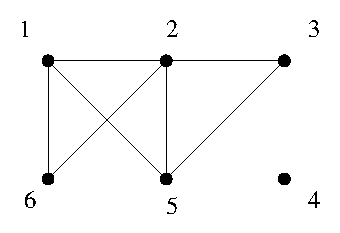
\includegraphics[width=0.3\textwidth]{images/02/graph01.eps}
    \end{tabular}
  \end{center}
  \caption*{\label{fig:ex:01} Grafo $G_1$.}
\end{figure}

% Página 7

%%%%%%%%%%%%%%%%%%%%%%%%%%%%%%%%%%%%%%%%%%%%%%%%%%%%%%%%%%%%
\section{Grafos dirigidos}
\label{sec:digraph}

\begin{easylist}
  & Grafo dirigido ou digrafo: $G(V,E)$ é um conjunto finito não vazio $V$ e um conjunto $E$ de pares ordenados de elementos de $V$. Portanto, em um digrafo, uma aresta $(v, w)$ possui uma única direção, de $v$ para $w$. Diz-se também que $(v, w)$ é divergente de $v$ e convergente a $w$. Caminhos e ciclos em um digrafo devem obedecer ao direcionamento das arestas. É possível haver ciclos de comprimento 2 quando $(v, w)$ e $(w, v)$ pertencem a $E$ simultaneamente.
  & Grafo subjacente: é uma versão não dirigida de $D(V, E)$, ou seja, o grafo obtido trocando-se os pares ordenados $(v, w)$ de $E$ por pares não ordenados.
  & Grau de entrada: número de arestas convergentes a $v$. Uma fonte é um vértice com grau de entrada nulo.
  & Grau de saída: número de arestas divergentes de $v$. Um sumidouro é um vértice com grau de saída nulo.
  & Digrafo fortemente conexo: é um digrafo $D(V, E)$ em que, para todo par de vértices $(v, w)$ existe caminho de $v$ para $w$ e também de $w$ para $v$.
  & Digrafo unilateralmente conexo: é um digrafo $D(V, E)$ em que, para todo par de vértices $(v, w)$ existe caminho de $v$ para $w$ e/ou de $w$ para $v$.
  & Digrafo fracamente conexo: é um digrafo $D(V, E)$ cujo grafo subjacente é conexo.
  & Digrafo desconexo: é um digrafo $D(V, E)$ cujo grafo subjacente é desconexo.
  & Fechamento transitivo: é o maior digrafo $D_f(V, E_f)$ que preserva a alcançabilidade de $D$.
  & Redução transitiva: é o menor digrafo $D_r(V, E_r)$ que preserva a alcançabilidade de $D$. Também é conhecida como diagrama de Hasse.

\begin{figure}[t]
  \begin{center}
    \begin{tabular}{c}
      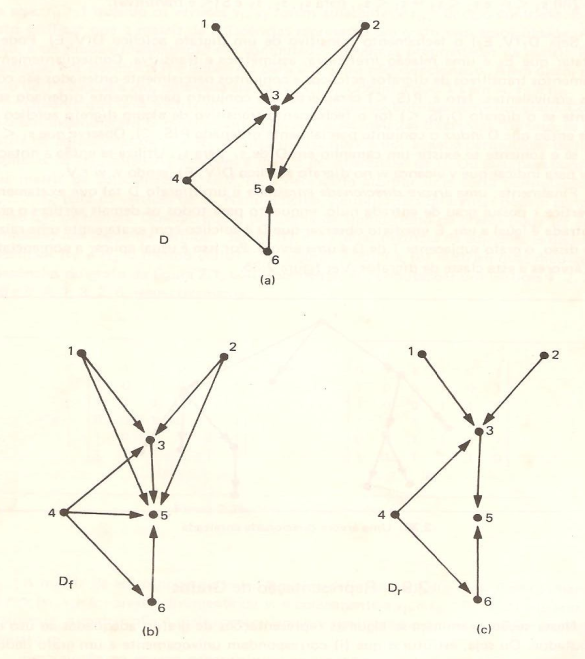
\includegraphics[width=0.7\textwidth]{images/02/digraph.png}
    \end{tabular}
  \end{center}
  \caption{\label{fig:1} (a) Um digrafo $D(V,E)$; (b) seu fechamento transitivo, e; (c) sua redução transitiva.}
  \source{Szwarcfiter~\cite{Szwarcfiter1986grafos}.}
\end{figure}

\clearpage

  & Conjunto parcialmente ordenado ou poset: denotado pelo par $(S, \leq)$, é um conjunto não vazio $S$ e uma relação binária $\leq$ em $S$ satisfazendo as seguintes propriedades:

%\end{easylist}

\begin{enumerate}
\item $s_1 \leq s_1$ para $s_1 \in S$ (reflexiva)

\item $s_1 \leq s_2$ e $s_2 \leq s_1 \Rightarrow s_1 = s_2$ para $s_1, s_2 \in S$ (anti-simétrica)

\item $s_1 \leq s_2$ e $s_2 \leq s_3 \Rightarrow s_1 \leq s_3$ para $s_1, s_2, s_3 \in S$ (transitiva)
\end{enumerate}

  && Um poset também pode ser definido pelo par $(S, <)$, onde $<$ é uma relação binária definida por $s_1 < s_2 \Leftrightarrow s_1\leq s_2$ e $s_1 \neq s_2$. A relação $<$ satisfaz as seguintes propriedades:


\begin{enumerate}
\item $s_1 \nless s_1$ para $s_1 \in S$ (irreflexiva)

\item $s_1 < s_2 \Rightarrow s_2 \nless s_1$ para $s_1, s_2 \in S$ (assimétrica)

\item $s_1 < s_2$ e $s_2 < s_3 \Rightarrow s_1 < s_3$ para $s_1, s_2, s_3 \in S$ (transitiva)
\end{enumerate}

  && Seja $D_f(V, E_f)$ o fechamento transitivo de um digrafo acíclico $D(V, E)$. Pode-se constatar qeu $E_f$ é uma relação irreflexiva, assimétrica e transitiva. Portanto, fechamentos transitivos e posets são conceitos equivalentes. Dizemos então que $D$ induz o conjunto parcialmente ordenado $P(V, <)$. Podemos dizer que $v<w$ em $P$ sse $v$ alcança $w$ em $D$, onde $v, w \in V$.

& Árvore dirigida enraizada: é um digrafo $D(V, E)$ tal que um vértice dito a raiz possui grau de entrada nulo, grau de saída não nulo, e todos os demais possuem grau de entrada igual a 1. Esse digrafo é acíclico e seu grafo subjacente é uma árvore.

\end{easylist}

\clearpage

%%%%%%%%%%%%%%%%%%%%%%%%%%%%%%%%%%%%%%%%%%%%%%%%%%%%%%%%%%%%
\section{Exercícios}

%$ \NOT \; \OR \; \AND \; \IMP \; \BIC$

\begin{enumerate}
  \item Para responder os itens a seguir, considere o grafo $G_2$ abaixo.
    \begin{enumerate}
      \item Encontre um caminho Hamiltoniano.
      \item Encontre um ciclo Hamiltoniano.
      \item Encontre um caminho Euleriano.
      \item Encontre um ciclo Euleriano em $G_2 - (5,8)$.
      \item Forneça uma lista de vértices que induza um conjunto indepentente de vértices.
      \item Forneça uma lista de vértices que induza um conjunto indepentente de vértices de tamanho 4.
      \item Forneça uma lista de vértices que induza um clique de tamanho 3.
      \item Forneça uma lista de vértices que induza um clique de tamanho 4.
      \item Forneça uma lista de vértices que induza um clique de tamanho 5.
      \item Quantas arestas possui uma árvore com todos os vértices de $G_2$?
      \item Dê um exemplo de árvore que seja um subgrafo de $G_2$.
      \item Forneça sua matriz de adjacências.
      \item Forneça sua matriz de incidências.
      \item Forneça sua estrutura de adjacências.
    \end{enumerate}

\begin{figure}[h!]
  \begin{center}
    \begin{tabular}{c}
      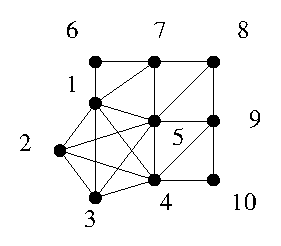
\includegraphics[width=0.3\textwidth]{images/02/ex01.eps}
    \end{tabular}
  \end{center}
  \caption*{\label{fig:ex:01} Grafo $G_2$.}
\end{figure}

  \item Forneça um algoritmo que recebe um grafo e um vértice como parâmetros, executa uma busca em largura e retorna uma lista de vértices na ordem em que foram percorridos.

  \item Forneça um algoritmo que recebe um grafo, um vértice $a$ e um vértice $b$ como parâmetros. Retorna o caminho mais curto entre $a$ e $b$.


\end{enumerate}

